\chapter{Financial Accounting}

\section{Introduction}

\begin{definition}
    [Accounting]
    Accounting is a measure of business activity that is communicated through financial statements and shared with investors, creditors, and other stakeholders.
\end{definition}

\begin{definition}
    [Managerial Accounting]
    Managerial accounting is the recording and analysis of financial information for internal use by management.
\end{definition}

\begin{definition}
    [Financial Accounting]
    Financial accounting is the process of recording financial information for external use by investors, creditors, tax authorities, and other stakeholders.\\
    \textbf{It is governed by Generally Accepted Accounting Principles (GAAP).}
\end{definition}

\begin{definition}
    [Proprietorship]
    A business owned by one person. This person has unlimited liability for the business.
\end{definition}

\begin{definition}
    [Partnership]
    A business owned by two or more people. Each partner has unlimited liability for the business.
\end{definition}

\begin{definition}
    [Corporation]
    A business that is a separate legal entity from its owners. The owners are shareholders who have limited liability for the business.
\end{definition}

\begin{definition}
    [Generally Accepted Accounting Principles (GAAP)]
    The objective of GAAP is to provide information useful for decision-making.\\
    The information must be:
    \begin{itemize}
        \item Relevant
        \item Reliable
        \item Comparable
    \end{itemize}
\end{definition}

\begin{theorem}
    [Accounting Principles]
    \begin{itemize}
        \item Entity Concept: Each entity is an economic unit that is separate from its owners.
        \item Relevance Characteristic: Information is relevant if it can influence a decision.
        \item Reliability/Objectivity Principle: Accounting information must be accurate and verifiable.
        \item Cost Principle: Assets are recorded at their actual cost (market value is variable, thus unreliable).
        \item Going-Concern Principle: Assumes the business will continue to operate for the foreseeable future.
        \item Stable Monetary Unit Principle: Assumes the value of money is stable over time.
    \end{itemize}
\end{theorem}

\subsection{Financial Statements}

\begin{theorem}
    [Financial Statements]
    \begin{itemize}
        \item Income Statement: Reports the sales and expenses of the business over a period of time.
        \item Balance Sheet: Reports the financial position of the business at a point in time.
        \item Statement of Cash Flows: Reports the cash inflows and outflows of the business over a period of time.
        \item Statement of Retained Earnings: Reports the changes in retained earnings over a period of time.
    \end{itemize}
    We will focus on the Income Statement and Balance Sheet.
\end{theorem}

\begin{figure}[H]
    \centering
    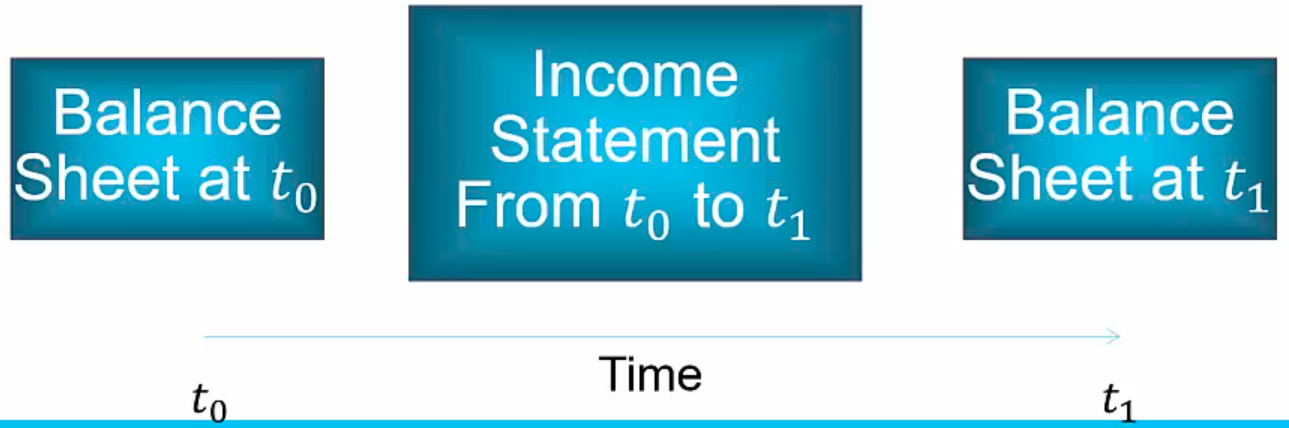
\includegraphics[width=0.8\textwidth]{LECTURE_8/balance-and-income.png}
    \caption{Balance Sheet and Income Statement}

\end{figure}

\begin{theorem}
    [The Accounting Equation]
    \begin{align}
        \text{Assets} & = \text{Liabilities} + \text{Owner's Equity} \\
        A             & = L + OE
    \end{align}
\end{theorem}

\begin{proposition}
    [Parts of the Balance Sheet]
    \begin{itemize}
        \item Assets: Resources owned by the business
        \item[] \begin{itemize}
                  \item Short-term assets: Cash, accounts receivable, inventory, Notes receivable, prepaid expenses
                  \item Long-term assets: Land, buildings, equipment, furniture, patents
              \end{itemize}
        \item Liabilities: Debts owed by the business
        \item[] \begin{itemize}
                  \item Short-term liabilities: Accounts payable, short-term loans
                  \item Long-term liabilities: Long-term loans
              \end{itemize}
        \item Owner's Equity: The owner's claim on the business
        \item[] \begin{itemize}
                  \item Paid In Equity: The amount the owner has invested in the business
                  \item Retained Earnings: The amount the business has earned and Retained
                  \item[] \begin{itemize}
                            \item This is the sum of all the net incomes the business has earned since it started, as stated in the previous income statements.
                        \end{itemize}
              \end{itemize}
    \end{itemize}
\end{proposition}

\begin{proposition}
    [Temporary Accounts]
    A temporary account is an account that is closed (reset to zero) at the end of the accounting period. Revenue and expenses are temporary accounts and get added to the retained earnings account at the end of the period.
\end{proposition}

\begin{proposition}
    [Parts of the Income Statement]
    \begin{itemize}
        \item Revenue: The amount earned from selling goods or services
        \item Expenses: The costs of doing business
        \item Net Income: Revenue - Expenses
    \end{itemize}
\end{proposition}

\begin{definition}
    [Accrual Accounting]
    Revenue is recorded when it is earned, and expenses are recorded when they are incurred. This means that revenue and expenses are recorded when they happen, not when the cash is received or paid.
\end{definition}

\begin{definition}
    [Cash Accounting]
    Revenue is recorded when cash is received, and expenses are recorded when cash is paid. This means that revenue and expenses are recorded when the cash is received or paid, not when they happen.\\
    In general, this is not a good method for accounting because it does not accurately reflect the current financial position of the business.
\end{definition}

\begin{definition}
    [Credits and Debits]
    \begin{itemize}
        \item Debits: Increase assets and expenses, decrease liabilities, revenue, and equity
        \item Credits: Increase liabilities, revenue, and equity, decrease assets and expenses
        \item The accounting equation must always balance
    \end{itemize}
\end{definition}

\begin{figure}[H]
    \centering
    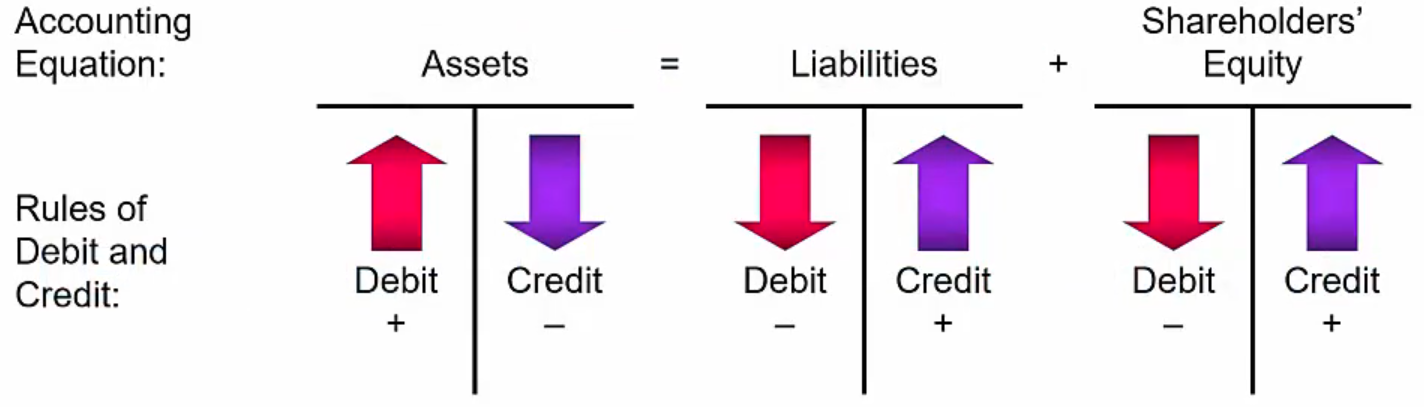
\includegraphics[width=0.8\textwidth]{LECTURE_8/credits-and-debits.png}
    \caption{Debits and Credits}

\end{figure}


\begin{remark}
    Remember that an increase in revenue increases equity (which is a right side item). This should mean that revenue is right side item.\\
\end{remark}

\section{Financial Ratios}

\begin{definition}
    [Financial Ratios]
    Financial ratios are used to analyze a company's financial health. They are interpreted by comparing them to the ratios of previous years, other companies, or industry averages.
\end{definition}

\begin{remark}
    This is a 'quick and dirty' way to analyze a company's financial health. Cash flow analysis is a more detailed way to analyze a company's financial health.
\end{remark}

\subsection{Liquidity Ratios}

\begin{definition}
    [Liquidity Ratios]
    Liquidity ratios measure a company's ability to pay off its short-term debts (within a year).
\end{definition}

\begin{theorem}
    [Current Ratio]
    \begin{align}
        \text{Current Ratio} & = \frac{\text{Current Assets}}{\text{Current Liabilities}}
    \end{align}
\end{theorem}

\begin{theorem}
    [Acid Test Ratio]
    A more aggressive measure of liquidity that only includes the most liquid assets.
    \begin{align}
        \text{Acid Test Ratio} & = \frac{\text{Cash} + \text{Short-term Investments} + \text{Net Current Receivables}}{\text{Current Liabilities}}
    \end{align}
\end{theorem}

\subsection{Inventory Ratios}

\begin{definition}
    [Inventory Ratios]
    Inventory ratios measure how efficiently a company to sell its inventory.
\end{definition}

\begin{theorem}
    [Inventory Turnover]
    \begin{align}
        \text{Inventory Turnover} & = \frac{\text{Cost of Goods Sold}}{\text{Average Inventory}}
    \end{align}
    \textbf{Note: This ratio will depend on the number of days being analyzed}
\end{theorem}

\begin{theorem}
    [Days' Inventory]
    \begin{align}
        \text{Days' Inventory} & = \frac{Average Inventory}{\text{Cost of Goods Sold in } t\text{ Days} / t}
    \end{align}
    \textbf{Note:} This is a normalized version of the Inventory Turnover ratio and \textbf{less is better.}
\end{theorem}
\section{Receivables Collection Ratios}
\begin{definition}
    [Receivables Collection Ratios]
    A measure of how quickly a company collects money from its customers.
\end{definition}

\begin{theorem}
    [Accounts Receivable Turnover]
    \begin{align}
        \text{Accounts Receivable Turnover} & = \frac{\text{Net Credit Sales}}{\text{Average Accounts Receivable}} \\
                                            & \text{OR}                                                            \\
        \text{Accounts Receivable Turnover} & = \frac{\text{Sales}}{\text{Average Accounts Receivable}}
    \end{align}
\end{theorem}

\begin{theorem}
    [Days' Receivables]
    \begin{align}
        \text{Days' Receivables} & = \frac{\text{Average Accounts Receivable}}{\text{Net Credit Sales in } t\text{ Days} / t} \\
                                 & \text{OR}                                                                                  \\
        \text{Days' Receivables} & = \frac{\text{Average Accounts Receivable}}{\text{Sales in } t\text{ Days} / t}
    \end{align}
    \textbf{Note:} This is a normalized version of the Accounts Receivable Turnover ratio and \textbf{less is better.}
\end{theorem}

\subsection{Leverage Ratios}

\begin{definition}
    [Leverage Ratios]
    Leverage ratios are a measure of a company's ability to pay, usually long-term, debt.
\end{definition}

\begin{theorem}
    [Debt Ratio]
    \begin{align}
        \text{Debt Ratio}   & = \frac{\text{Total Liabilities}}{\text{Total Assets}} \\
        \text{Equity Ratio} & = 1 - \text{Debt Ratio}                                \\
                            & = \frac{\text{Total Equity}}{\text{Total Assets}}
    \end{align}
    \textbf{Note:} Lower is better.
\end{theorem}

\begin{proposition}
    [Interpretation of the Debt Ratio]

    If two companies perform the same, but one has a higher debt ratio, the stakeholders of the more indebted company are taking on more risk and thus should expect a higher return. But the greater the debt ratio, the greater the risk of bankruptcy where shareholders equity is wiped out.
\end{proposition}

\begin{theorem}
    [Times-Interest-Earned]
    this is a measure of the number of times operating income can cover interest expense.
    \begin{align}
        \text{Times-Interest-Earned} & = \frac{\text{Income from Operations}}{\text{Interest Expense}}                    \\
                                     & \text{OR}                                                                          \\
        \text{Times-Interest-Earned} & = \frac{\text{Expenses Before Taxes and Interest (EBIT)}}{\text{Interest Expense}}
    \end{align}
    \textbf{Note:} Higher is better.
\end{theorem}

\subsection{Profitability Ratios}

\begin{theorem}
    [Profit Margin]
    \begin{align}
        \text{Profit Margin} & = \frac{\text{Net Income}}{\text{Sales}}
    \end{align}
\end{theorem}

\begin{theorem}
    [Return on Assets (ROA)]
    This is a measure of how profitability a company uses its assets.
    \begin{align}
        \text{ROA} & = \frac{\text{Net Income}}{\text{Total Assets}}                                      \\
                   & \text{OR}                                                                            \\
        \text{ROA} & = \frac{\text{Net Income} + \text{Interest}(1-\text{Tax Rate)}}{\text{Total Assets}}
    \end{align}

\end{theorem}

\begin{theorem}
    [Return on Equity (ROE)]
    A measure of how much the company has earned on funds invested by shareholders (directly and through retained earnings).
    \begin{align}
        \text{ROE} & = \frac{\text{Net Income}}{\text{Total Equity}}
    \end{align}
\end{theorem}

\begin{definition}
    [Shares Outstanding]
    The number of shares of a company that are traded on the stock market.
\end{definition}

\begin{theorem}
    [Earnings Per Share (EPS)]
    Profitability on a per-share basis.
    \begin{align}
        \text{EPS} & = \frac{\text{Net Income}}{\text{Total Shares Outstanding}}
    \end{align}
\end{theorem}

\subsection{Performance Ratios (Analysis of Shares)}

\begin{theorem}
    [Price-Earnings Ratio (P/E)]
    A measure of how much investors are willing to pay for a company's earnings.
    \begin{align}
        \text{P/E} & = \frac{\text{Price per Share}}{\text{Earnings per Share}}
    \end{align}
    \begin{itemize}
        \item A high P/E ratio indicates that investors expect higher earnings growth in the future or that the company is overvalued.
        \item Companies without earnings or that are losing money will not have a $P/E$ ratio.
        \item There is a positive relationship between debt and $P/E$ ratio, so be careful when comparing companies.
    \end{itemize}
\end{theorem}

\begin{theorem}
    [Dividend Yield]
    A measure of how much a company pays out in dividends each year relative to its share price.
    \begin{align}
        \text{Dividend Yield} & = \frac{\text{Dividends per Share}}{\text{Price per Share}}
    \end{align}
    \begin{itemize}
        \item Mature and stable companies are most likely to pay dividends.
        \item High growth companies typically reinvest earnings to grow the company.
    \end{itemize}
\end{theorem}

\begin{theorem}
    [Market Capitalization]
    The total value of a company's outstanding shares. This is not a ratio.
    \begin{align}
        \text{Market Capitalization} & = \text{Price per Share} \times \text{Total Shares Outstanding}
    \end{align}
\end{theorem}